\section{Theoretical Algebra}
\label{sect:result:theoretical_algebra}
In this section, a collection of XQuery query examples and their translation to
relational algebra is presented. The translation is done manually using the
``Tainting Dependencies'' method described in section
\ref{sect:trans:taintingDependencies}. For the sake of brevity, only the
rules used throughout the translation will be noted. Intermediate results will
not be included.

Generell struktur:
- Sp\oe rring
- Semantikk (resultat)
- Translasjon
- Mellomregninger? (naaii..)

\subsection{Extensive FLWOR}
This example will illustrate the translation of a more complex FLWOR expression.

\subsubsection{Query premise}
\begin{figure}[!htp]
\begin{center}
\begin{Verbatim}
for $a in (1,2,3) let $b := 2
  where $a gt $b
  order by $a
  return ($a, $b)
\end{Verbatim}
  \caption{Extensive FLWOR expression, showcasing for-, let-, where-, orderby-,
  and return-clauses}
  \label{fig:results:query_ext_flwor}
\end{center}
\end{figure}

\subsubsection{Translation process}
The translation process in its entirety is shown step by step in appendix
\ref{appendix:transl:ext_flwor}, page \pageref{appendix:transl:ext_flwor}.

\subsubsection{Result}
The result of the translation is shown in figure
\ref{fig:results:query_ext_flwor_result}.

\begin{figure}[!htp]
\begin{center}
  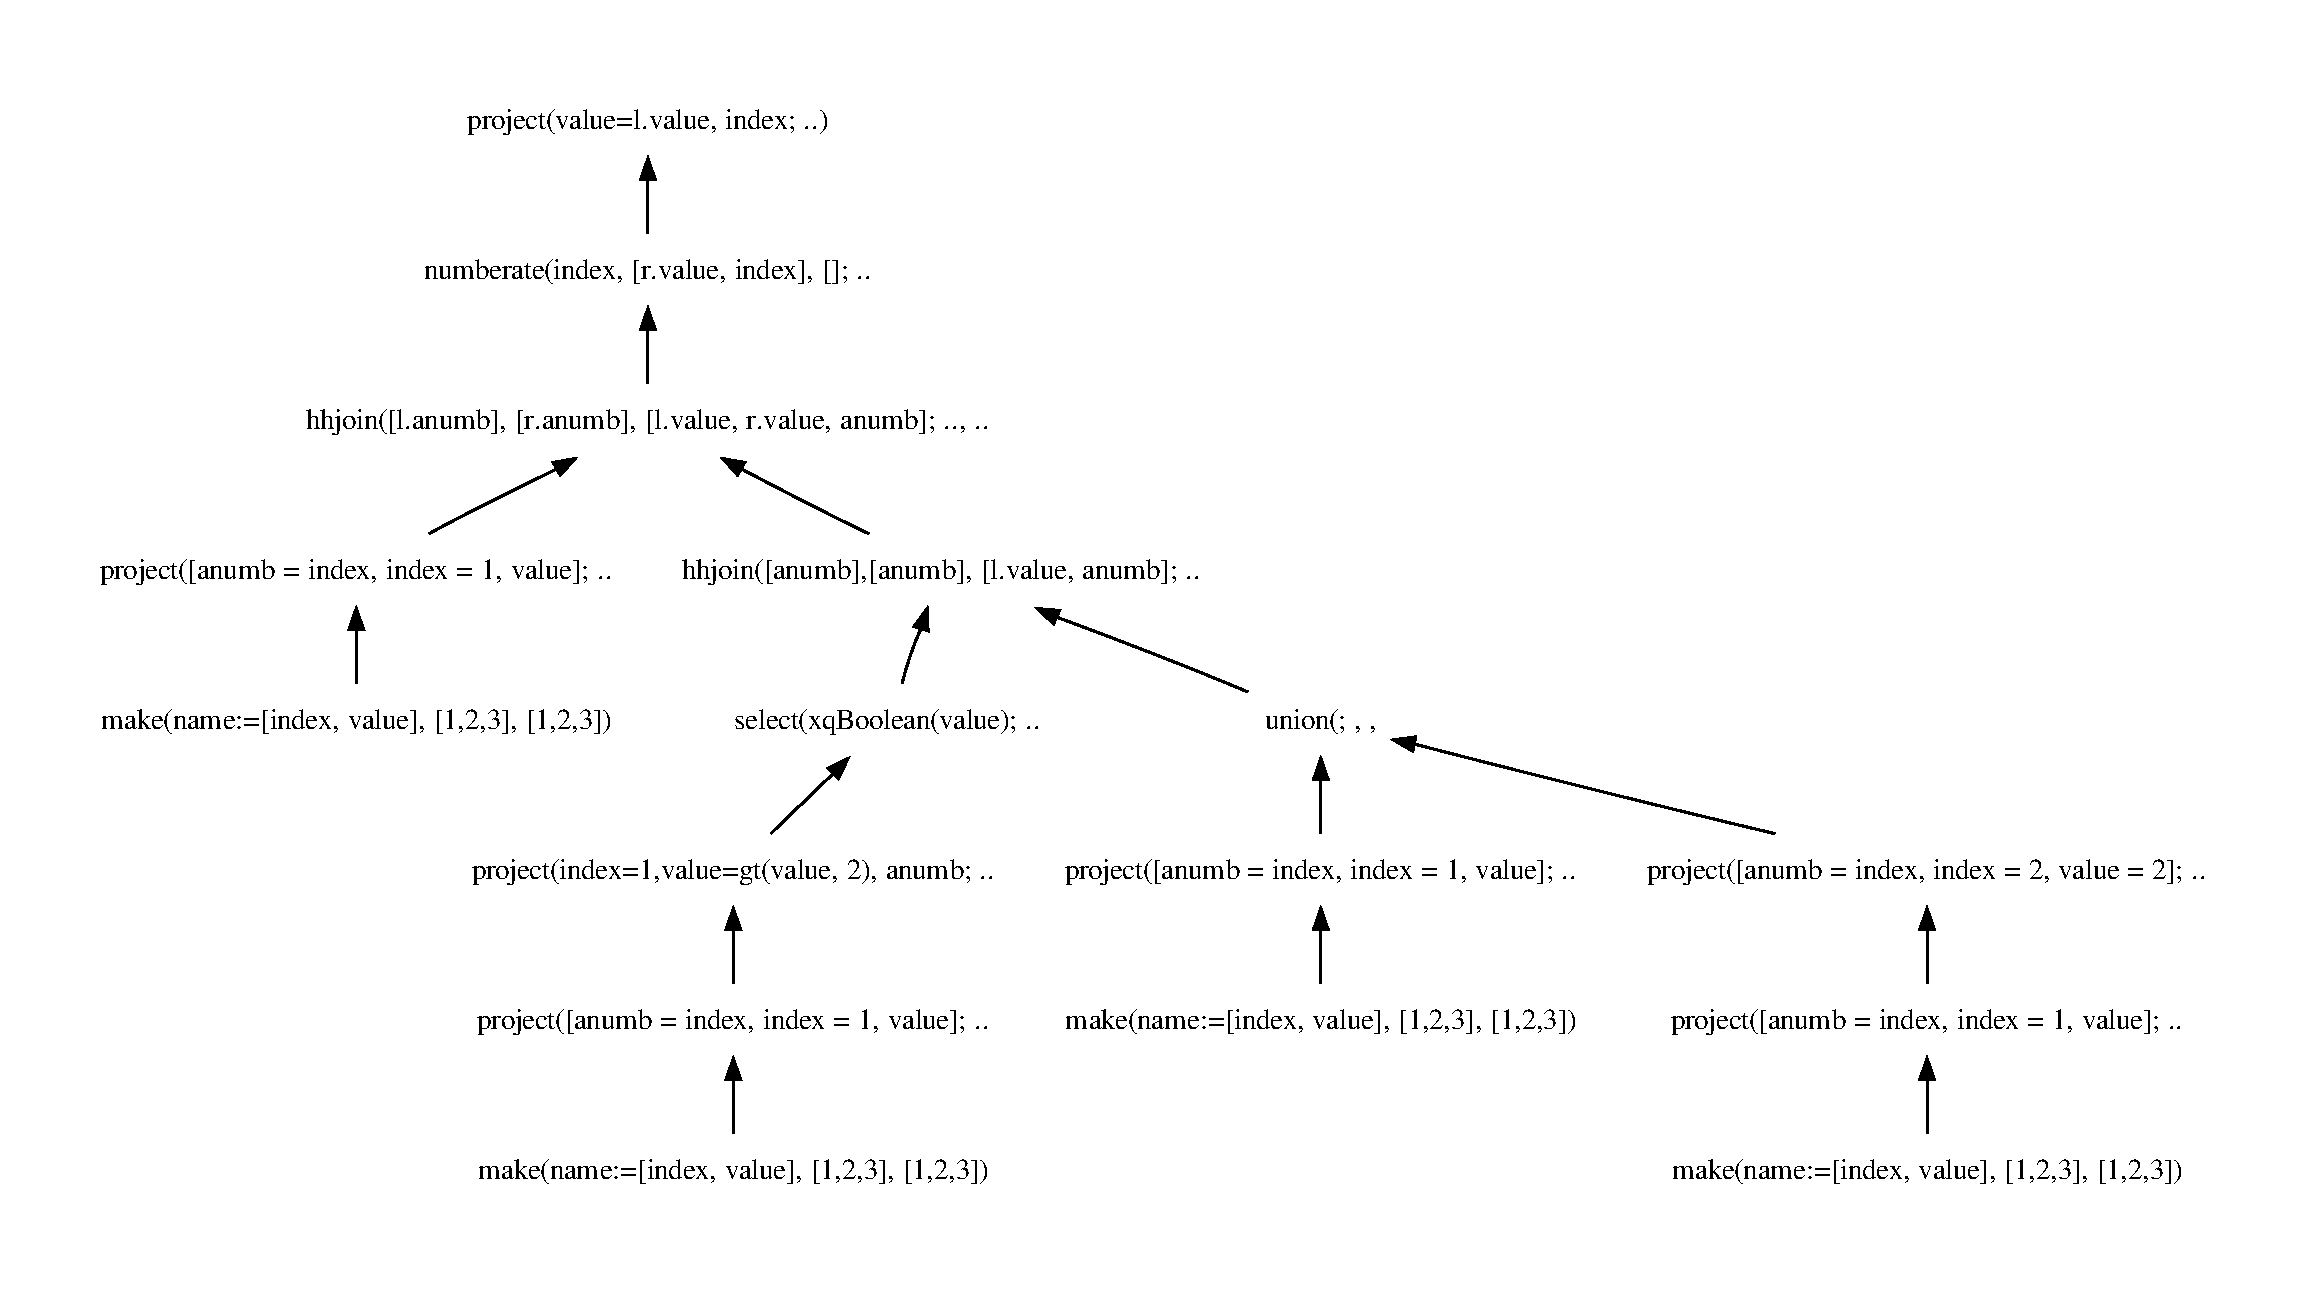
\includegraphics[width=1.0\textwidth]{img/graphs/ext_flwor}
  \caption{Complete translation of expression in figure
  \ref{fig:results:query_ext_flwor}}
  \label{fig:results:query_ext_flwor_result}
\end{center}
\end{figure}

The operator tree in figure \ref{fig:results:query_ext_flwor_result} can be
converted to the DAG seen in figure \ref{fig:results:query_ext_flwor_dag}.

\newpage

\begin{figure}[!htp]
\begin{center}
  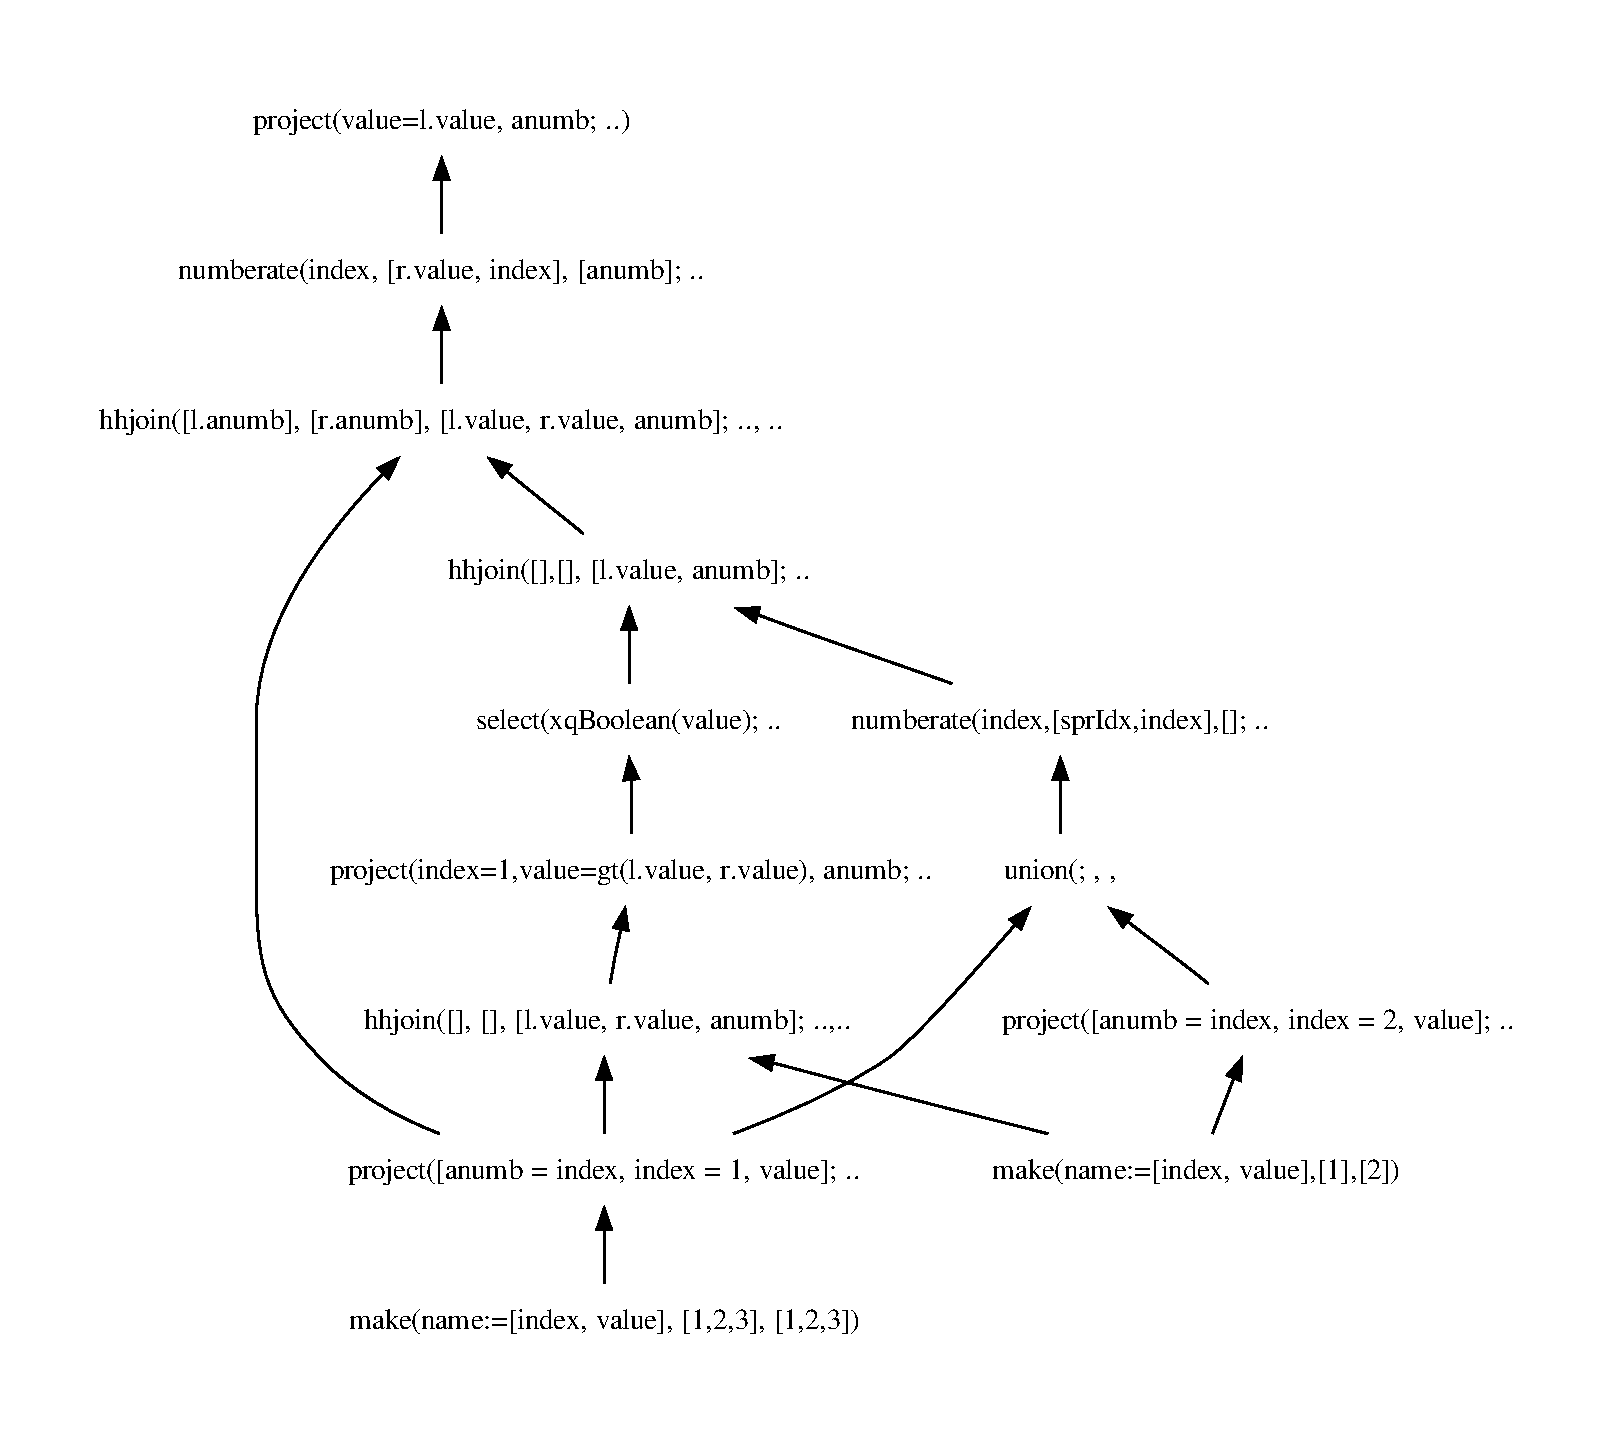
\includegraphics[width=1.0\textwidth]{img/graphs/ext_flwor_dag}
  \caption{DAG representation of operator tree in figure
  \ref{fig:results:query_ext_flwor_result}}
  \label{fig:results:query_ext_flwor_dag}
\end{center}
\end{figure}

\subsection{Path expression with predicate}
This example will illustrate the translation of a path expression with a predicate.

\subsubsection{Query premise}
\begin{figure}[!htp]
\begin{center}
\begin{Verbatim}
/a/b[@id eq 2] 
\end{Verbatim}
  \caption{Path expression with a predicate query premise}
  \label{fig:results:query_pathPred}
\end{center}
\end{figure}

\subsubsection{Translation process}
The translation process in its entirety is shown step by step in appendix
\ref{appendix:transl:pathPred}, page \pageref{appendix:transl:pathPred}.

\subsubsection{Result}
The result of the translation is shown in figure
\ref{fig:results:query_pathpred_result}.

\begin{figure}[!htp]
\begin{center}
  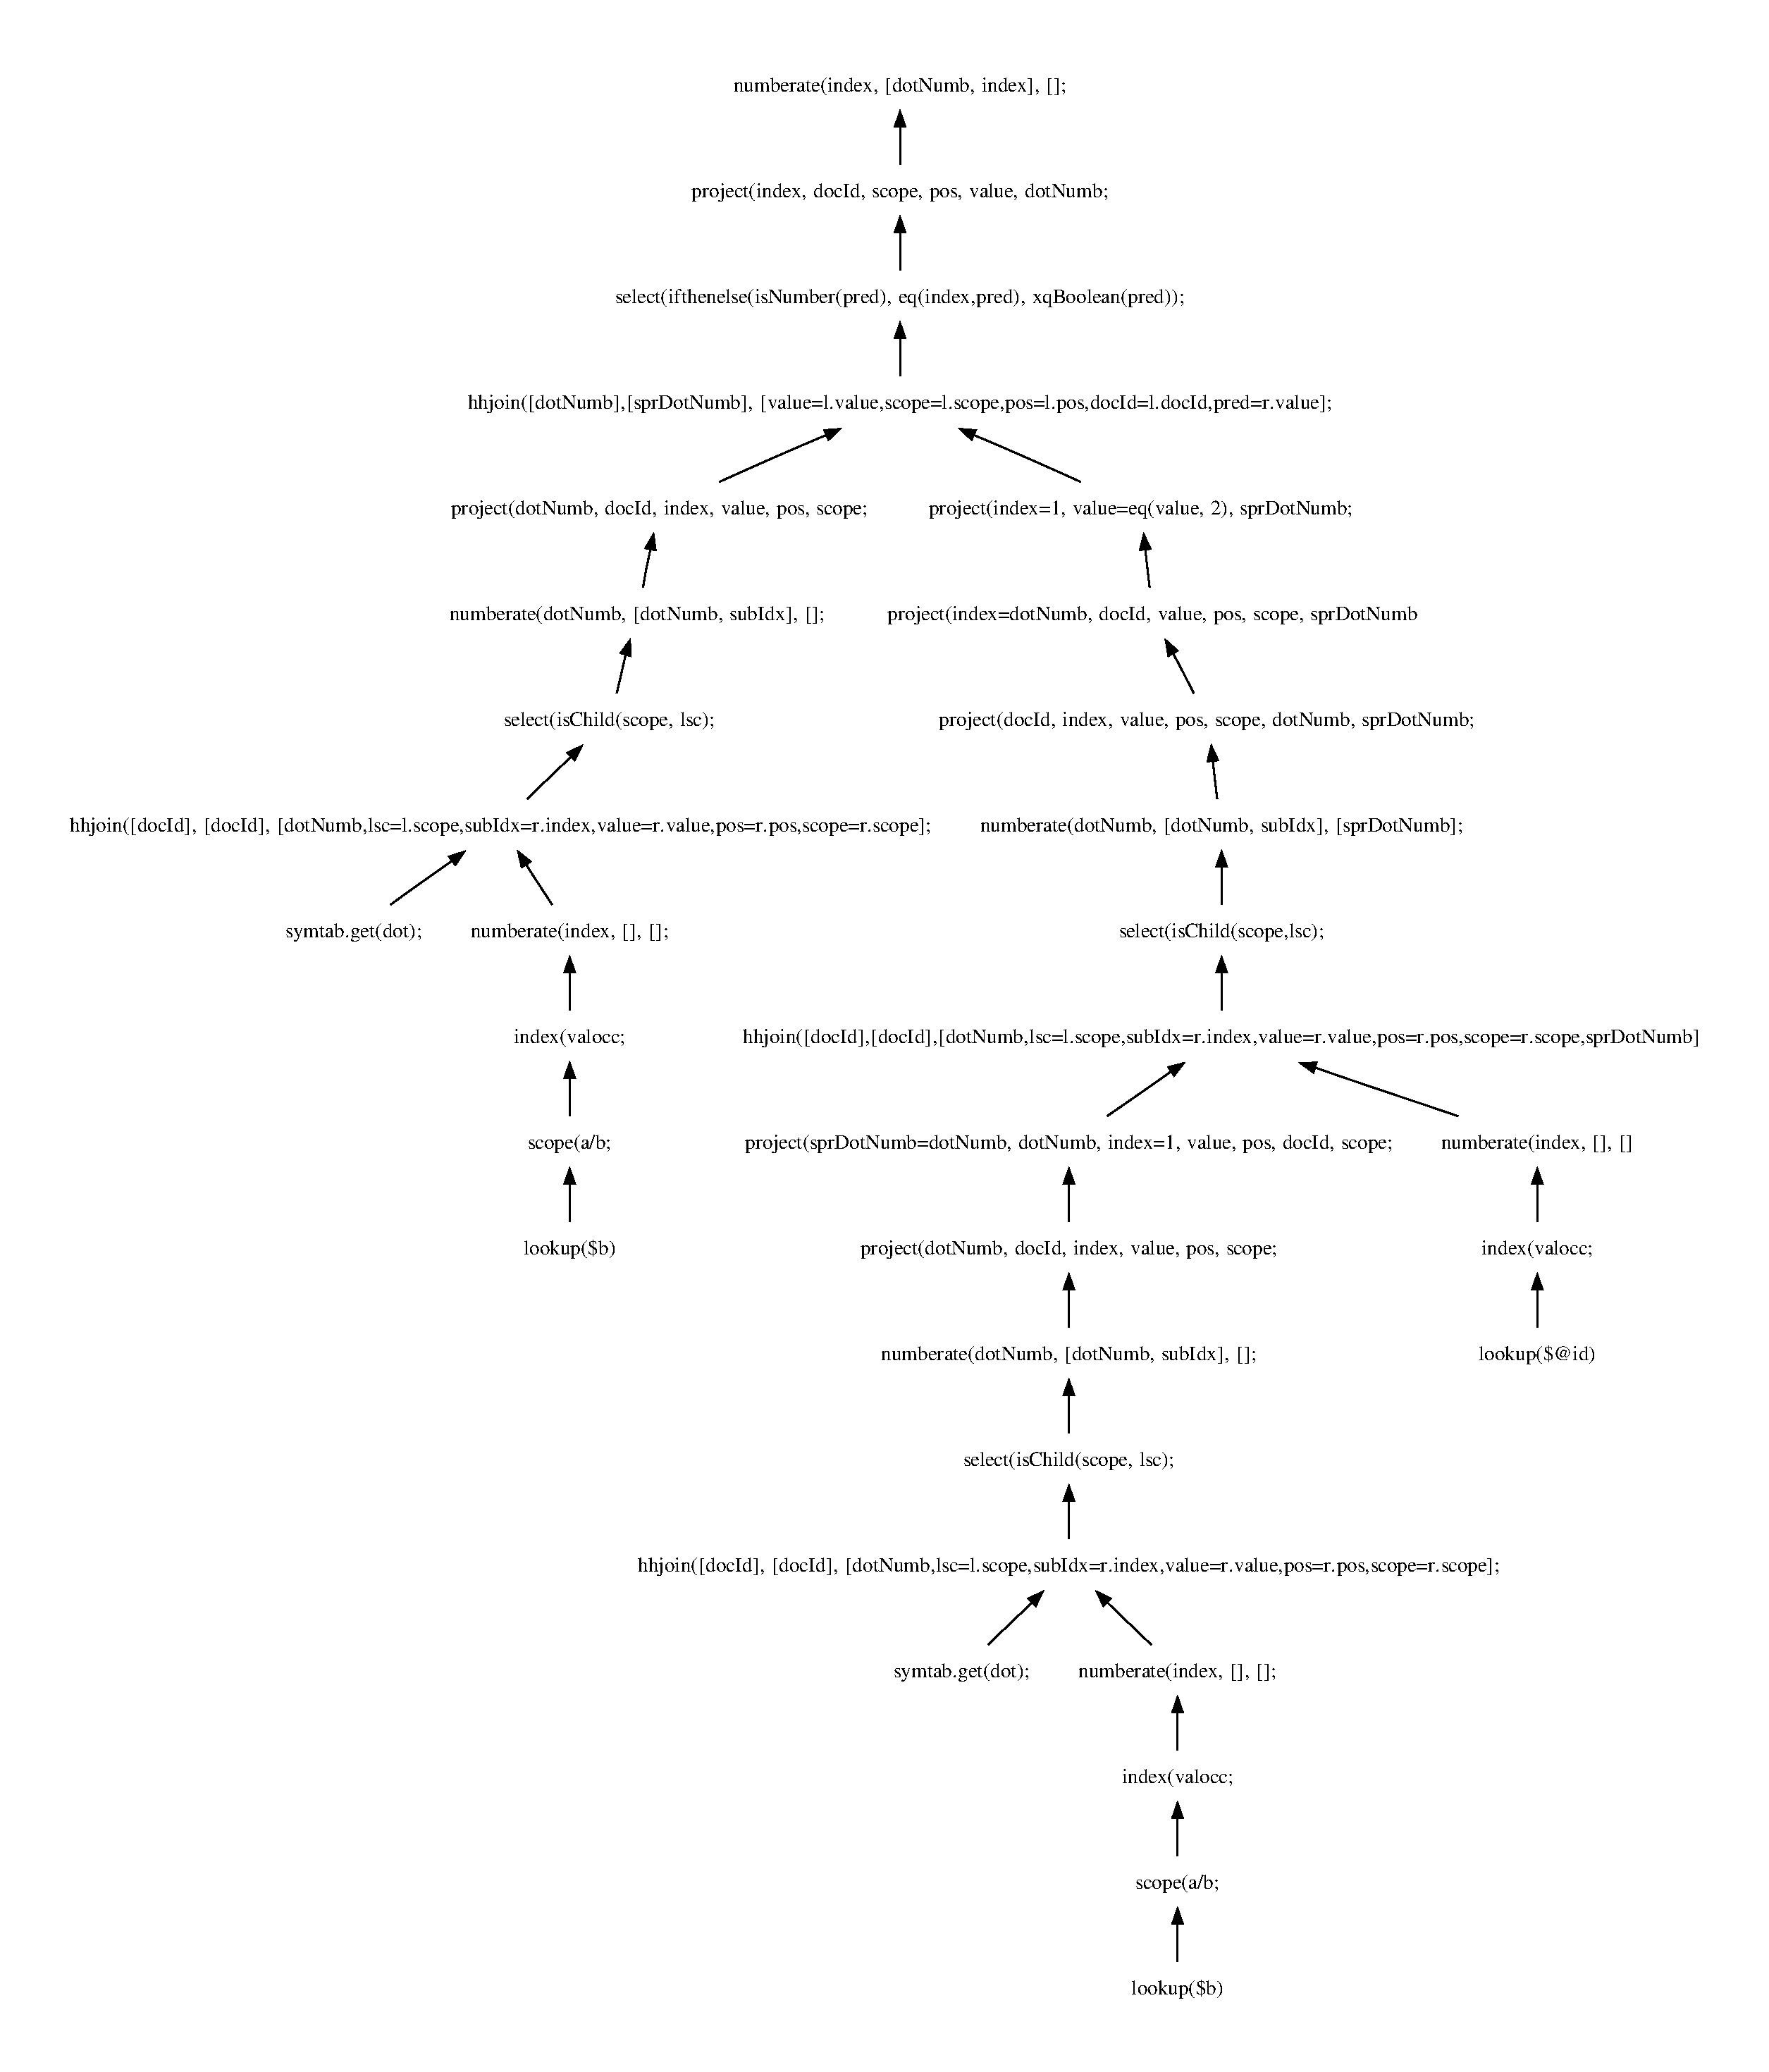
\includegraphics[width=1.0\textwidth]{img/graphs/TD_patExprPred}
  \caption{Complete translation of expression in figure
  \ref{fig:results:query_pathPred}}
  \label{fig:results:query_pathpred_result}
\end{center}
\end{figure}

The operator tree in figure \ref{fig:results:query_pathpred_result} can be
converted to the DAG seen in figure \ref{fig:results:query_pathpred_result_dag}.

\newpage

\begin{figure}[!htp]
\begin{center}
  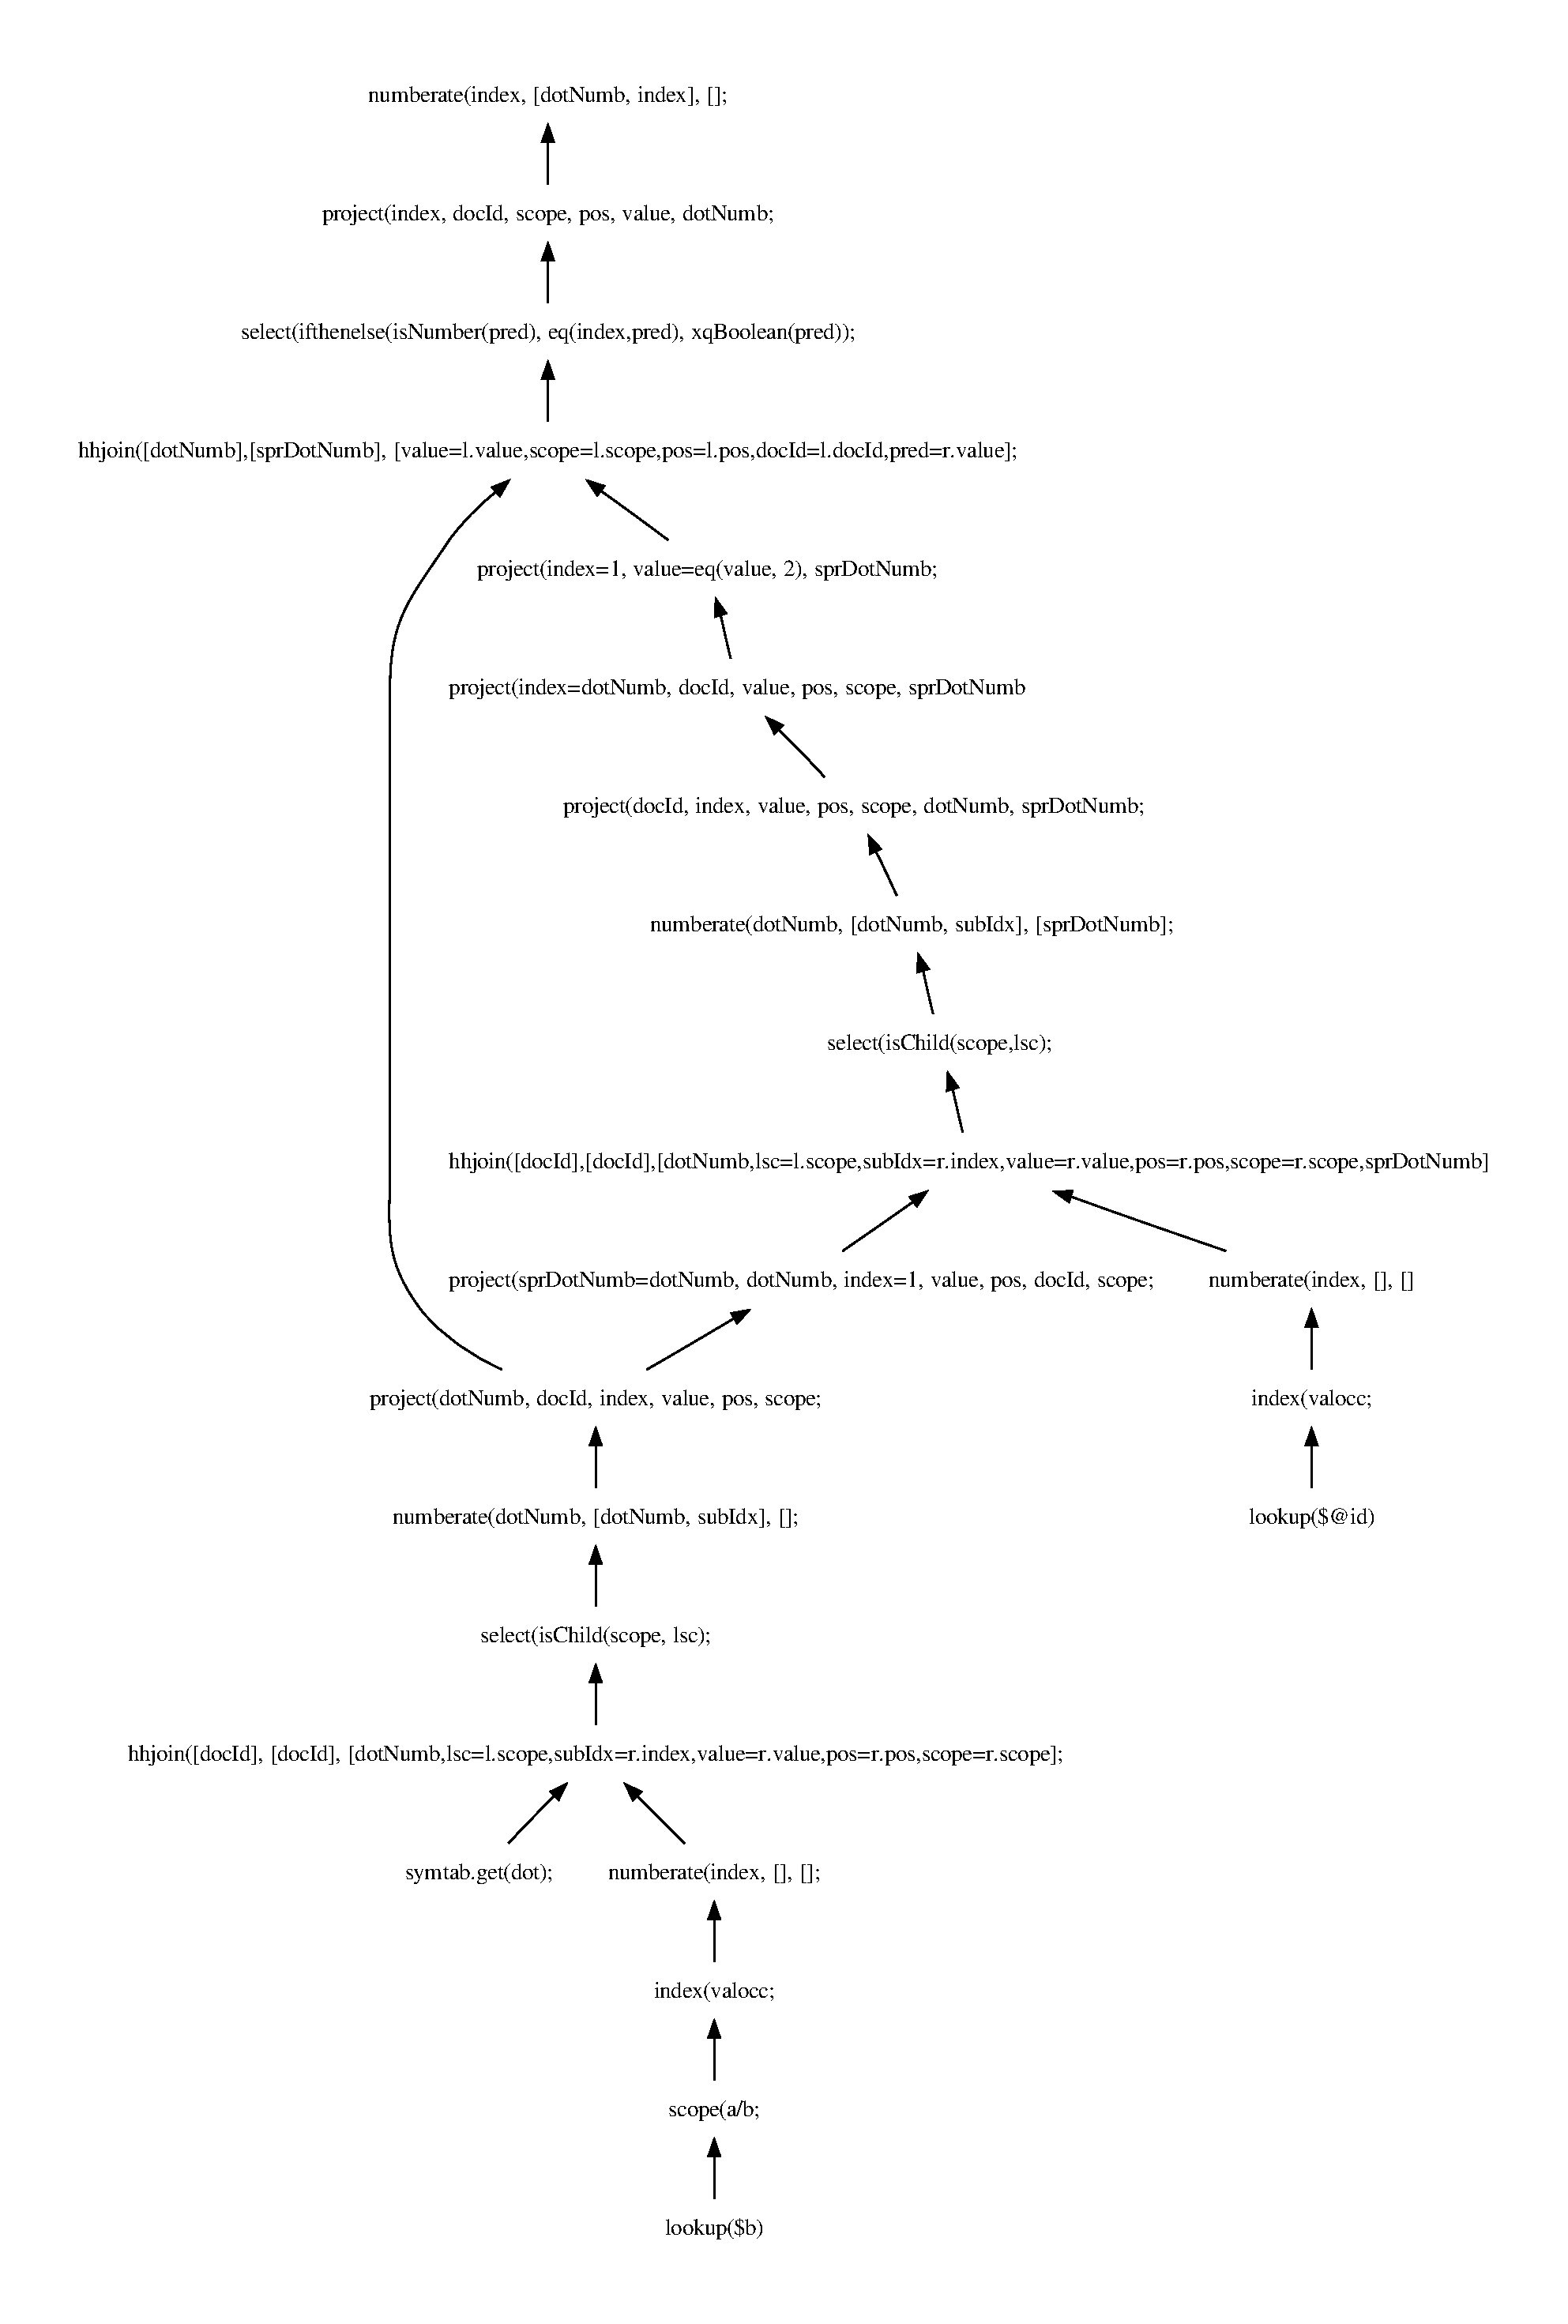
\includegraphics[width=1.0\textwidth]{img/graphs/TD_patExprPred_dag}
  \caption{DAG representation of operator tree in figure
  \ref{fig:results:query_pathpred_result}}
  \label{fig:results:query_pathpred_result_dag}
\end{center}
\end{figure}

\subsection{If-then-else}
\subsubsection{Query premise}
\begin{figure}[!htp]
\begin{center}
\begin{Verbatim}
for $a in (1,2,3) return
  if $a gt 2 then $a else 3
\end{Verbatim}
  \caption{If-then-else query premise}
  \label{fig:results:query_ifthenelse}
\end{center}
\end{figure}

\subsubsection{Translation process}
The translation process in its entirety is shown step by step in appendix
\ref{appendix:transl:ifthenelse}, page \pageref{appendix:transl:ifthenelse}.

\subsubsection{Result}
The result of the translation is shown in figure
\ref{fig:results:query_ifthenelse_result}.

\begin{figure}[!htp]
\begin{center}
  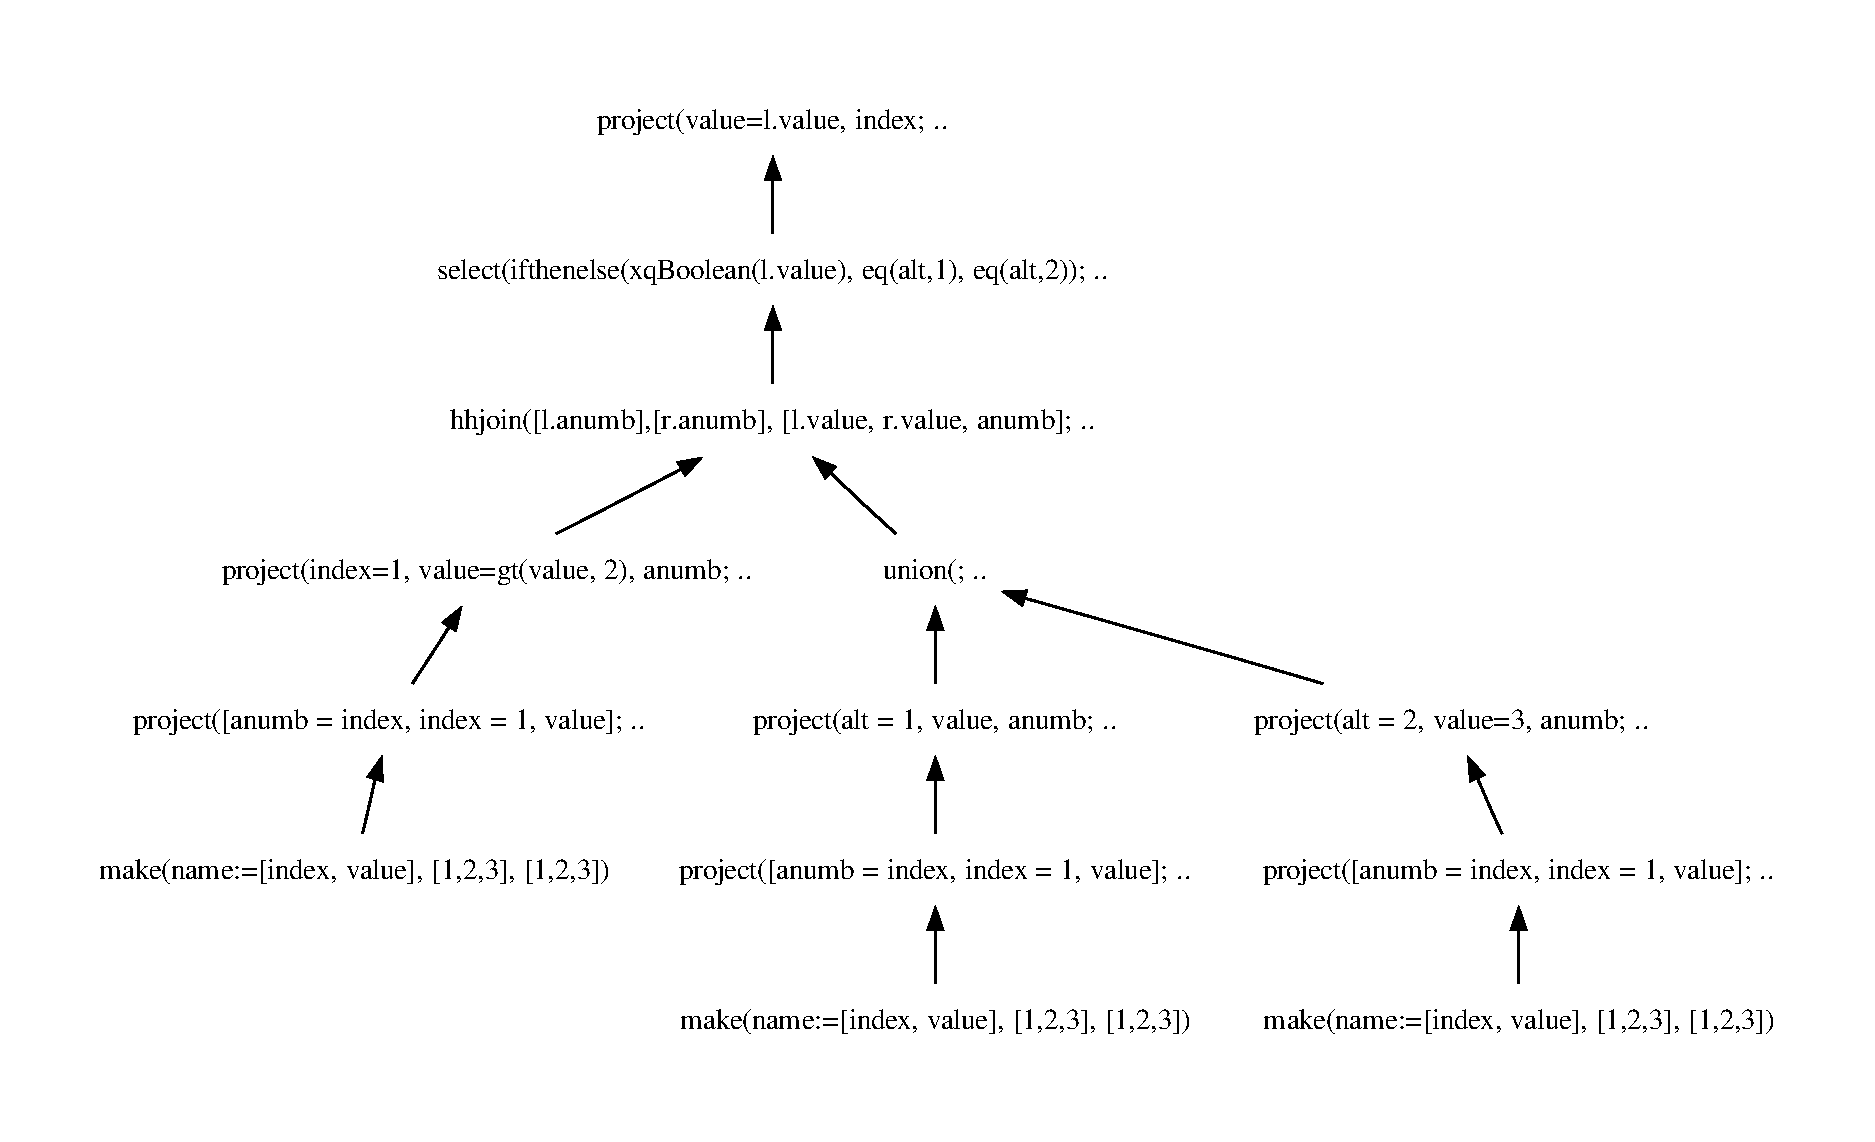
\includegraphics[width=1.0\textwidth]{img/graphs/ifthenelse}
  \caption{Complete translation of expression in figure
  \ref{fig:results:query_ifthenelse}}
  \label{fig:results:query_ifthenelse_result}
\end{center}
\end{figure}

The operator tree in figure \ref{fig:results:query_ifthenelse_result} can be
converted to the DAG seen in figure \ref{fig:results:query_ifthenelse_result_dag}.

\newpage

\begin{figure}[!htp]
\begin{center}
  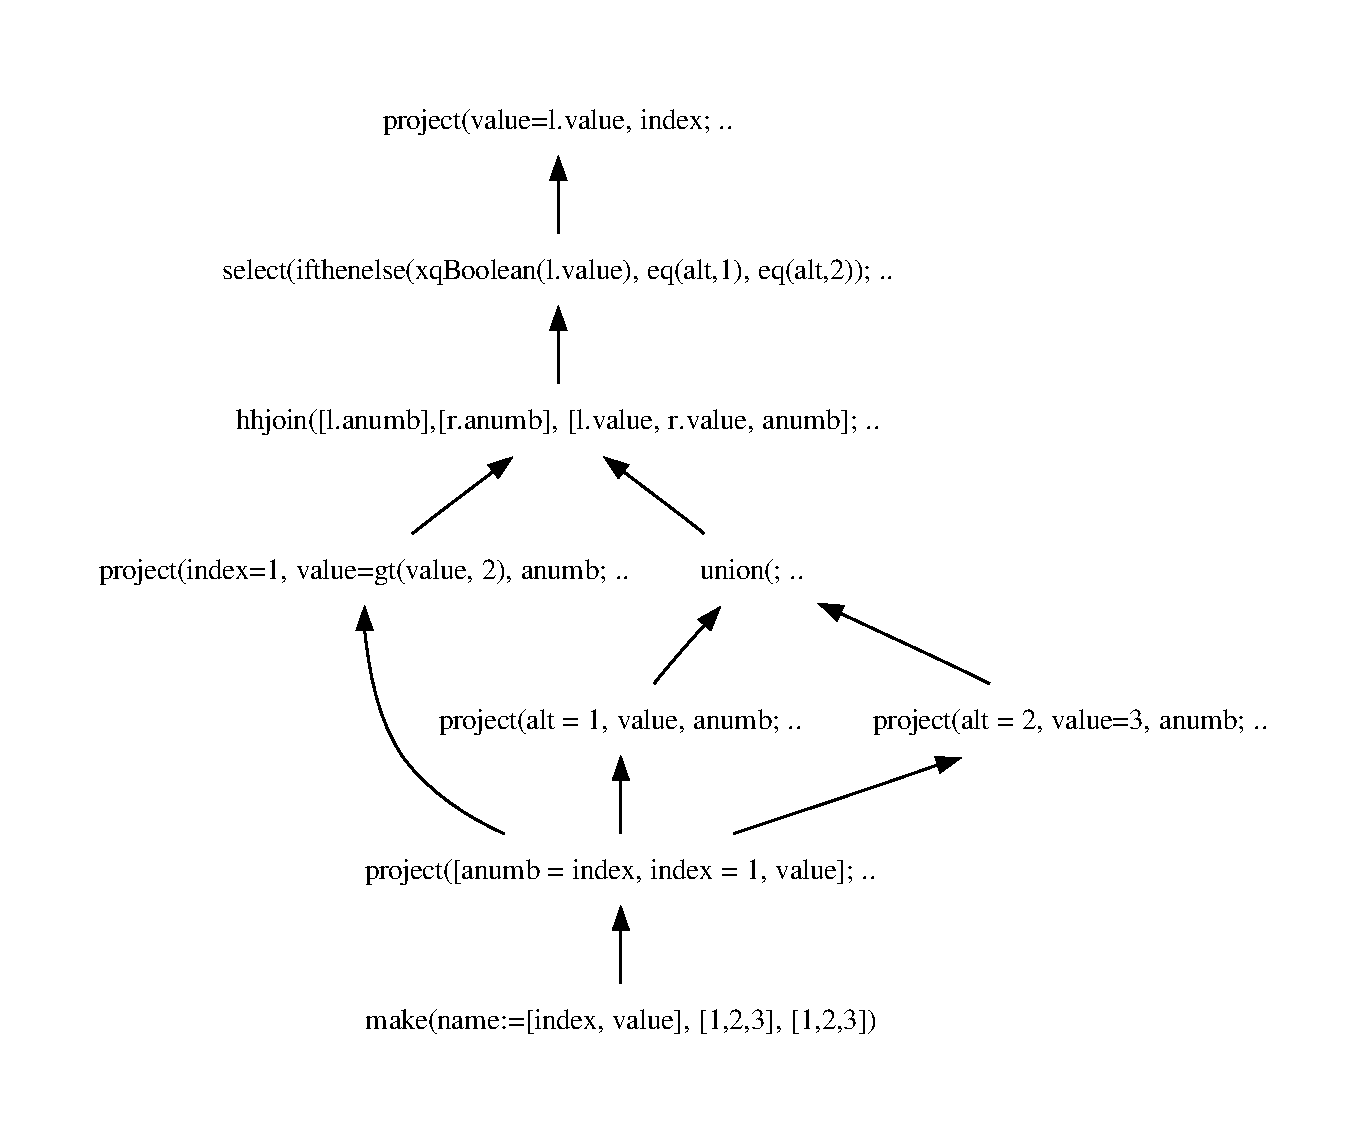
\includegraphics[width=1.0\textwidth]{img/graphs/ifthenelse_dag}
  \caption{DAG representation of operator tree in figure
  \ref{fig:results:query_ifthenelse_result}}
  \label{fig:results:query_ifthenelse_result_dag}
\end{center}
\end{figure}

\newpage

\section{Algebra Generated By Implementation}
\label{sect:result:implementation_algebra}
In this section, a collection of trivial queries are translated to relational
algebra using the implemented proof of concept described in chapter
\ref{chapter:implementation}. Naturally, this implementation also uses the
``Tainting Dependencies'' method, however the results from these translations
can also be used in a comparison with loop lifting.

\subsection{Trivial FLWOR}
\label{sect:results:algebra:generated:trivial_flwor}
\subsubsection{Query premise}
\begin{figure}[!htp]
\begin{center}
\begin{Verbatim}
for $a in (1,2,3) return $a
\end{Verbatim}
  \caption{Trivial FLWOR query premise}
  \label{fig:results:query_trivial_flwor}
\end{center}
\end{figure}

\subsubsection{Result}
\begin{figure}[!htp]
\begin{center}
  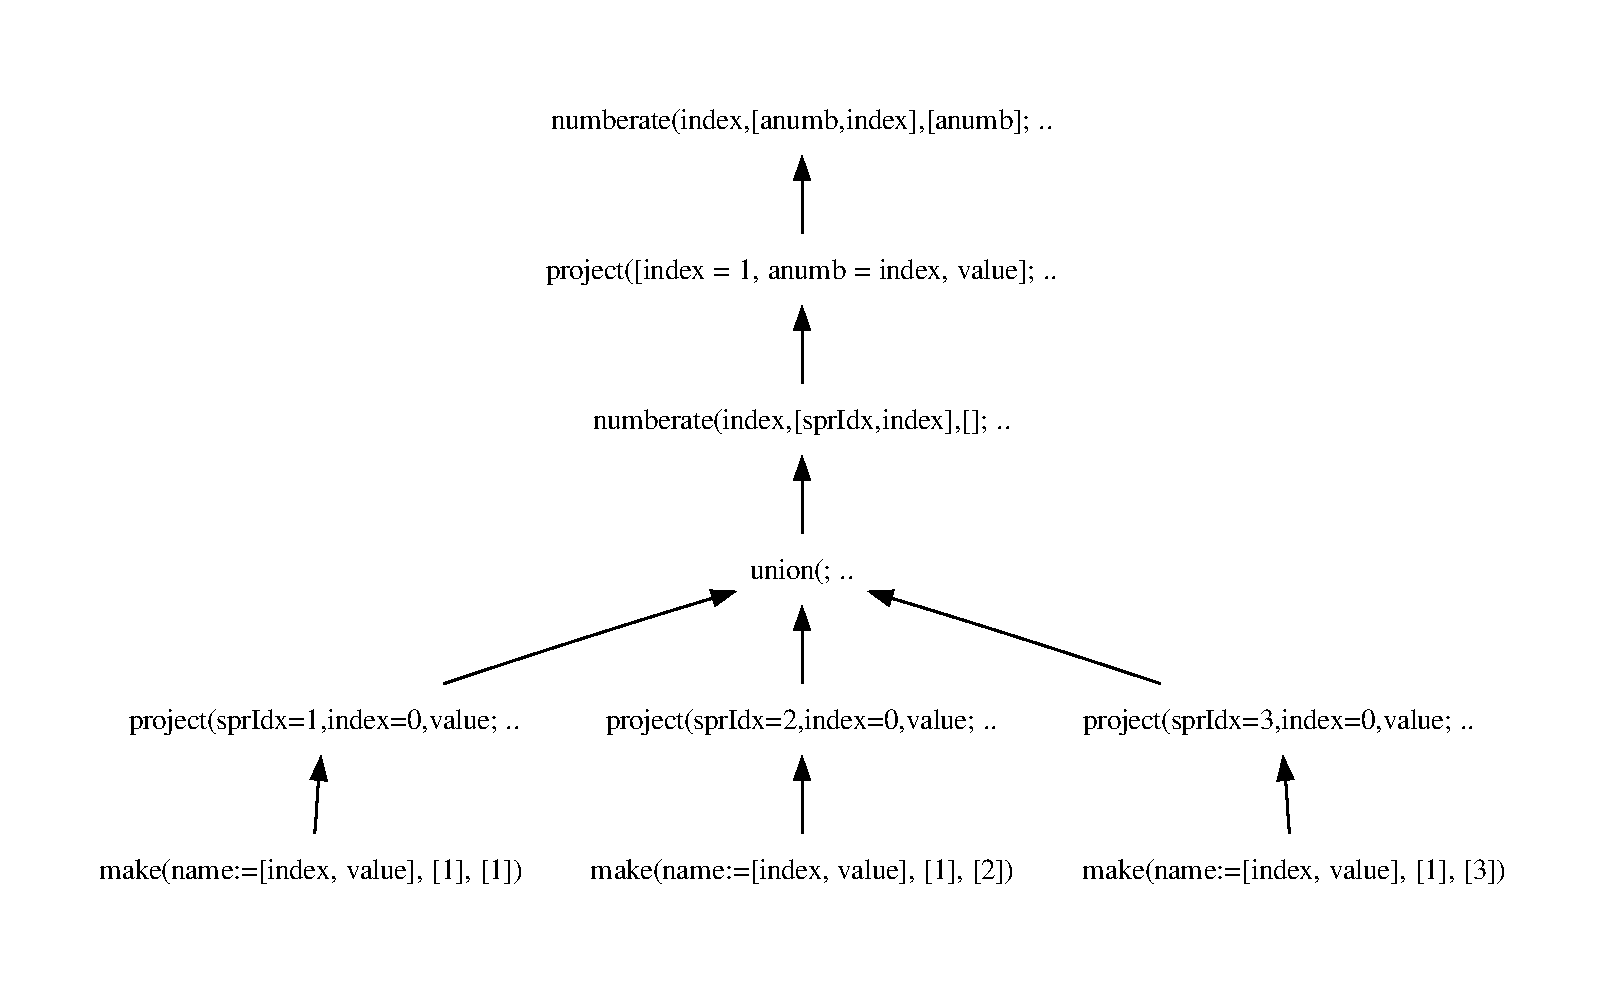
\includegraphics[width=1.0\textwidth]{img/graphs/td_impl_flwor_simple_xq_relalg} \caption{Complete translation of expression in figure
  \ref{fig:results:query_trivial_flwor}}
  \label{fig:results:query_trivial_flwor_result}
\end{center}
\end{figure}

\subsection{Complex FLWOR}
\label{sect:results:algebra:generated:complex_flwor}
\subsubsection{Query premise}
\begin{figure}[!htp]
\begin{center}
\begin{Verbatim}
for $a in (1,2) return (3, for $b in (4,5) return ($a, $b, 6))
\end{Verbatim}
  \caption{Complex FLWOR query premise}
  \label{fig:results:query_complex_flwor}
\end{center}
\end{figure}

\subsubsection{Result}
\begin{figure}[!htp]
\begin{center}
  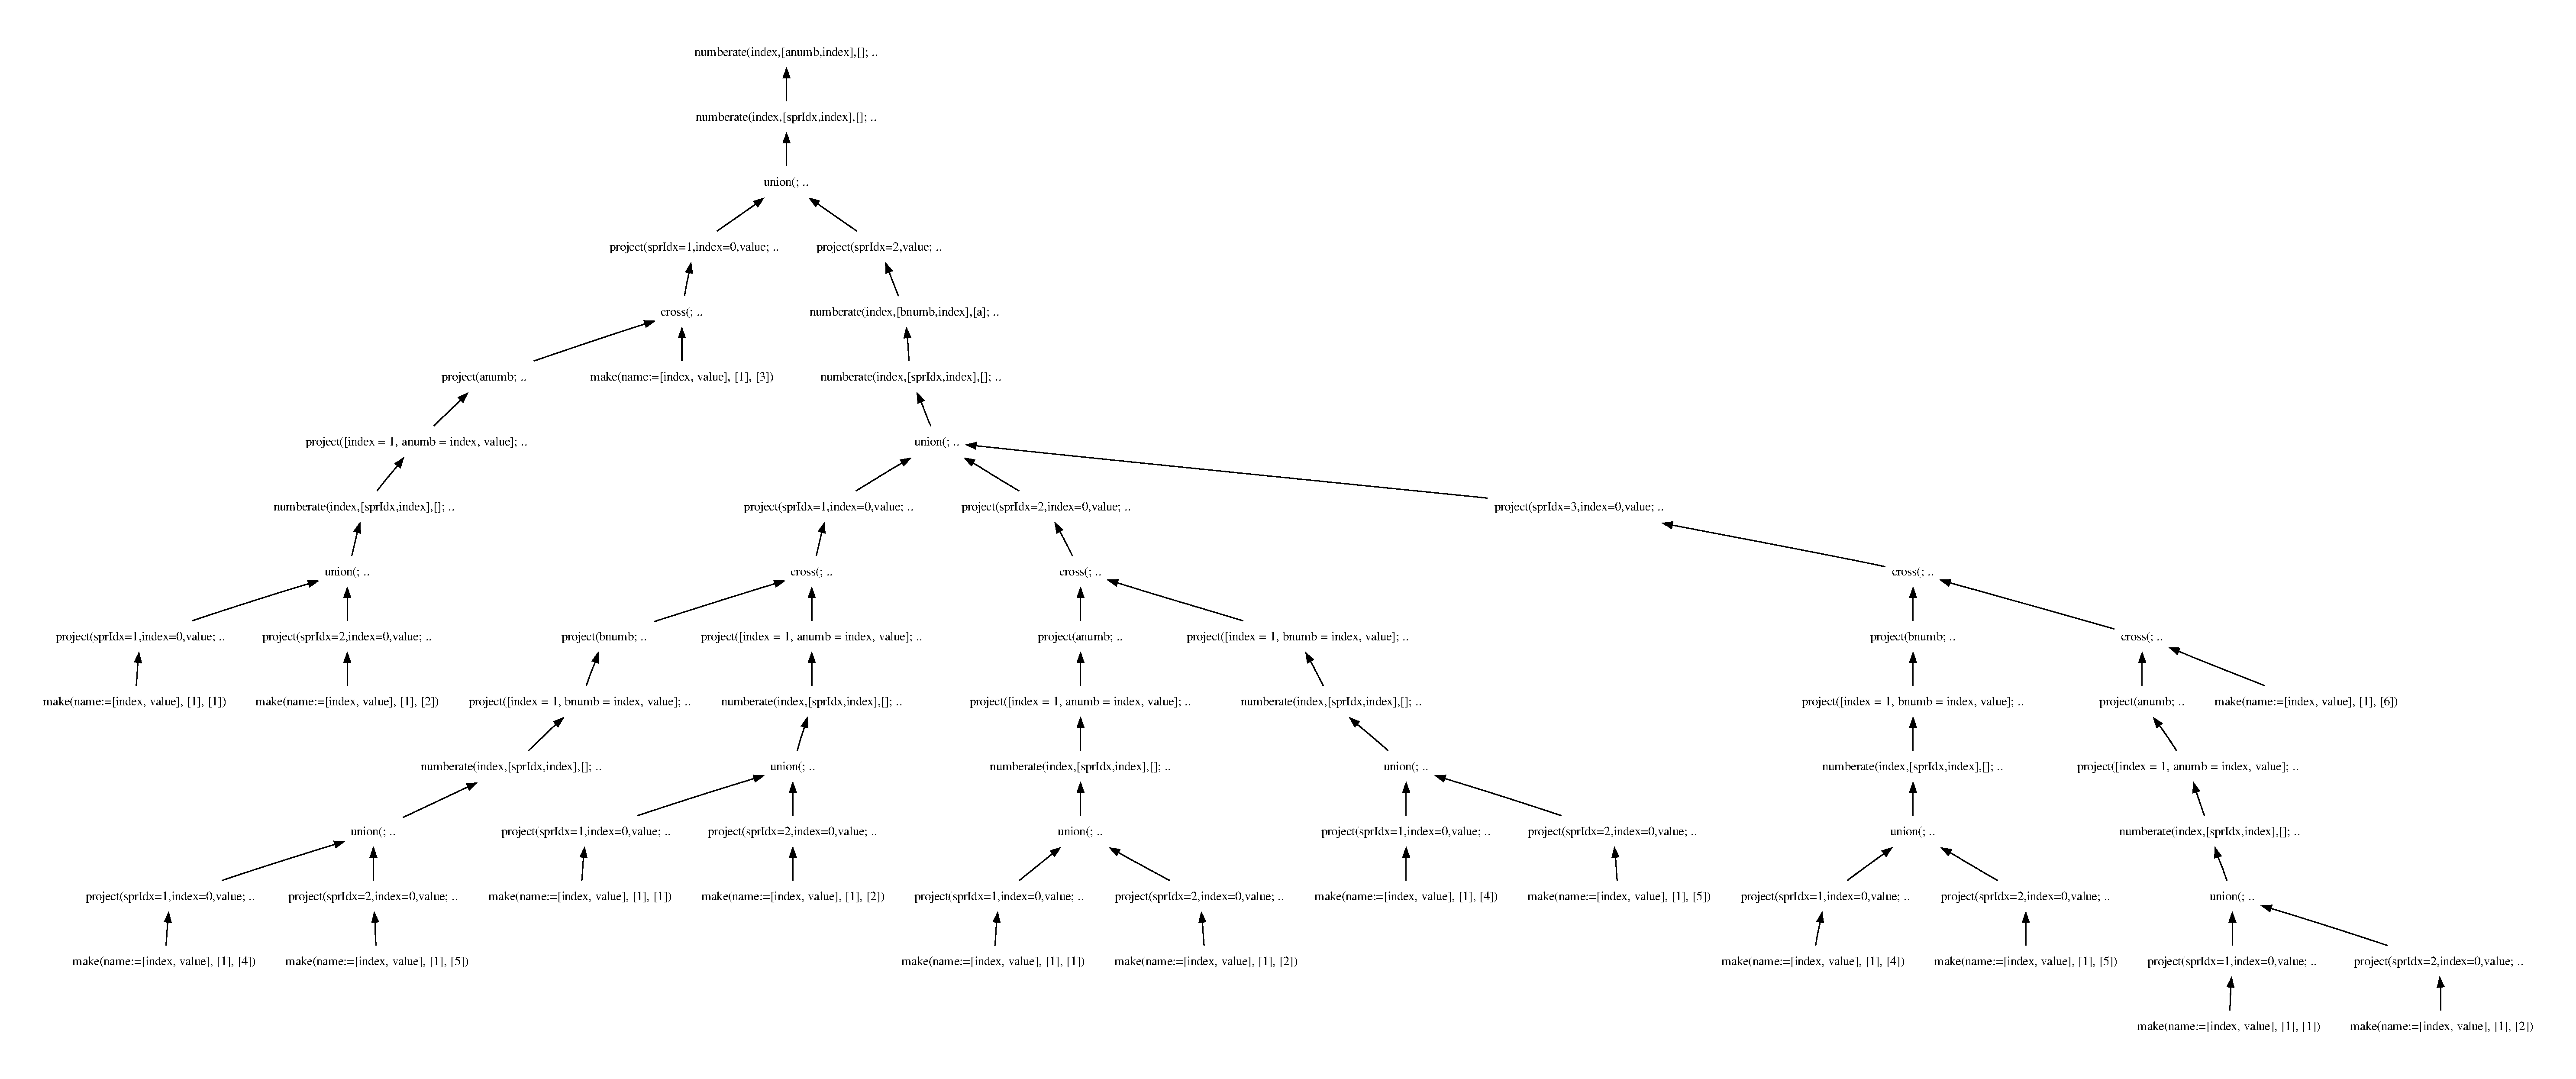
\includegraphics[angle=90,height=0.7\textheight]{img/graphs/td_impl_flwor_complex_xq_relalg} \caption{Complete
  translation of expression in figure
  \ref{fig:results:query_complex_flwor}}
  \label{fig:results:query_complex_flwor_result}
\end{center}
\end{figure}


The algebra tree in figure \ref{fig:results:query_complex_flwor_result} can
be converted to the DAG in figure
\ref{fig:results:query_complex_flwor_result_dag}

\begin{figure}[!htp]
\begin{center}
  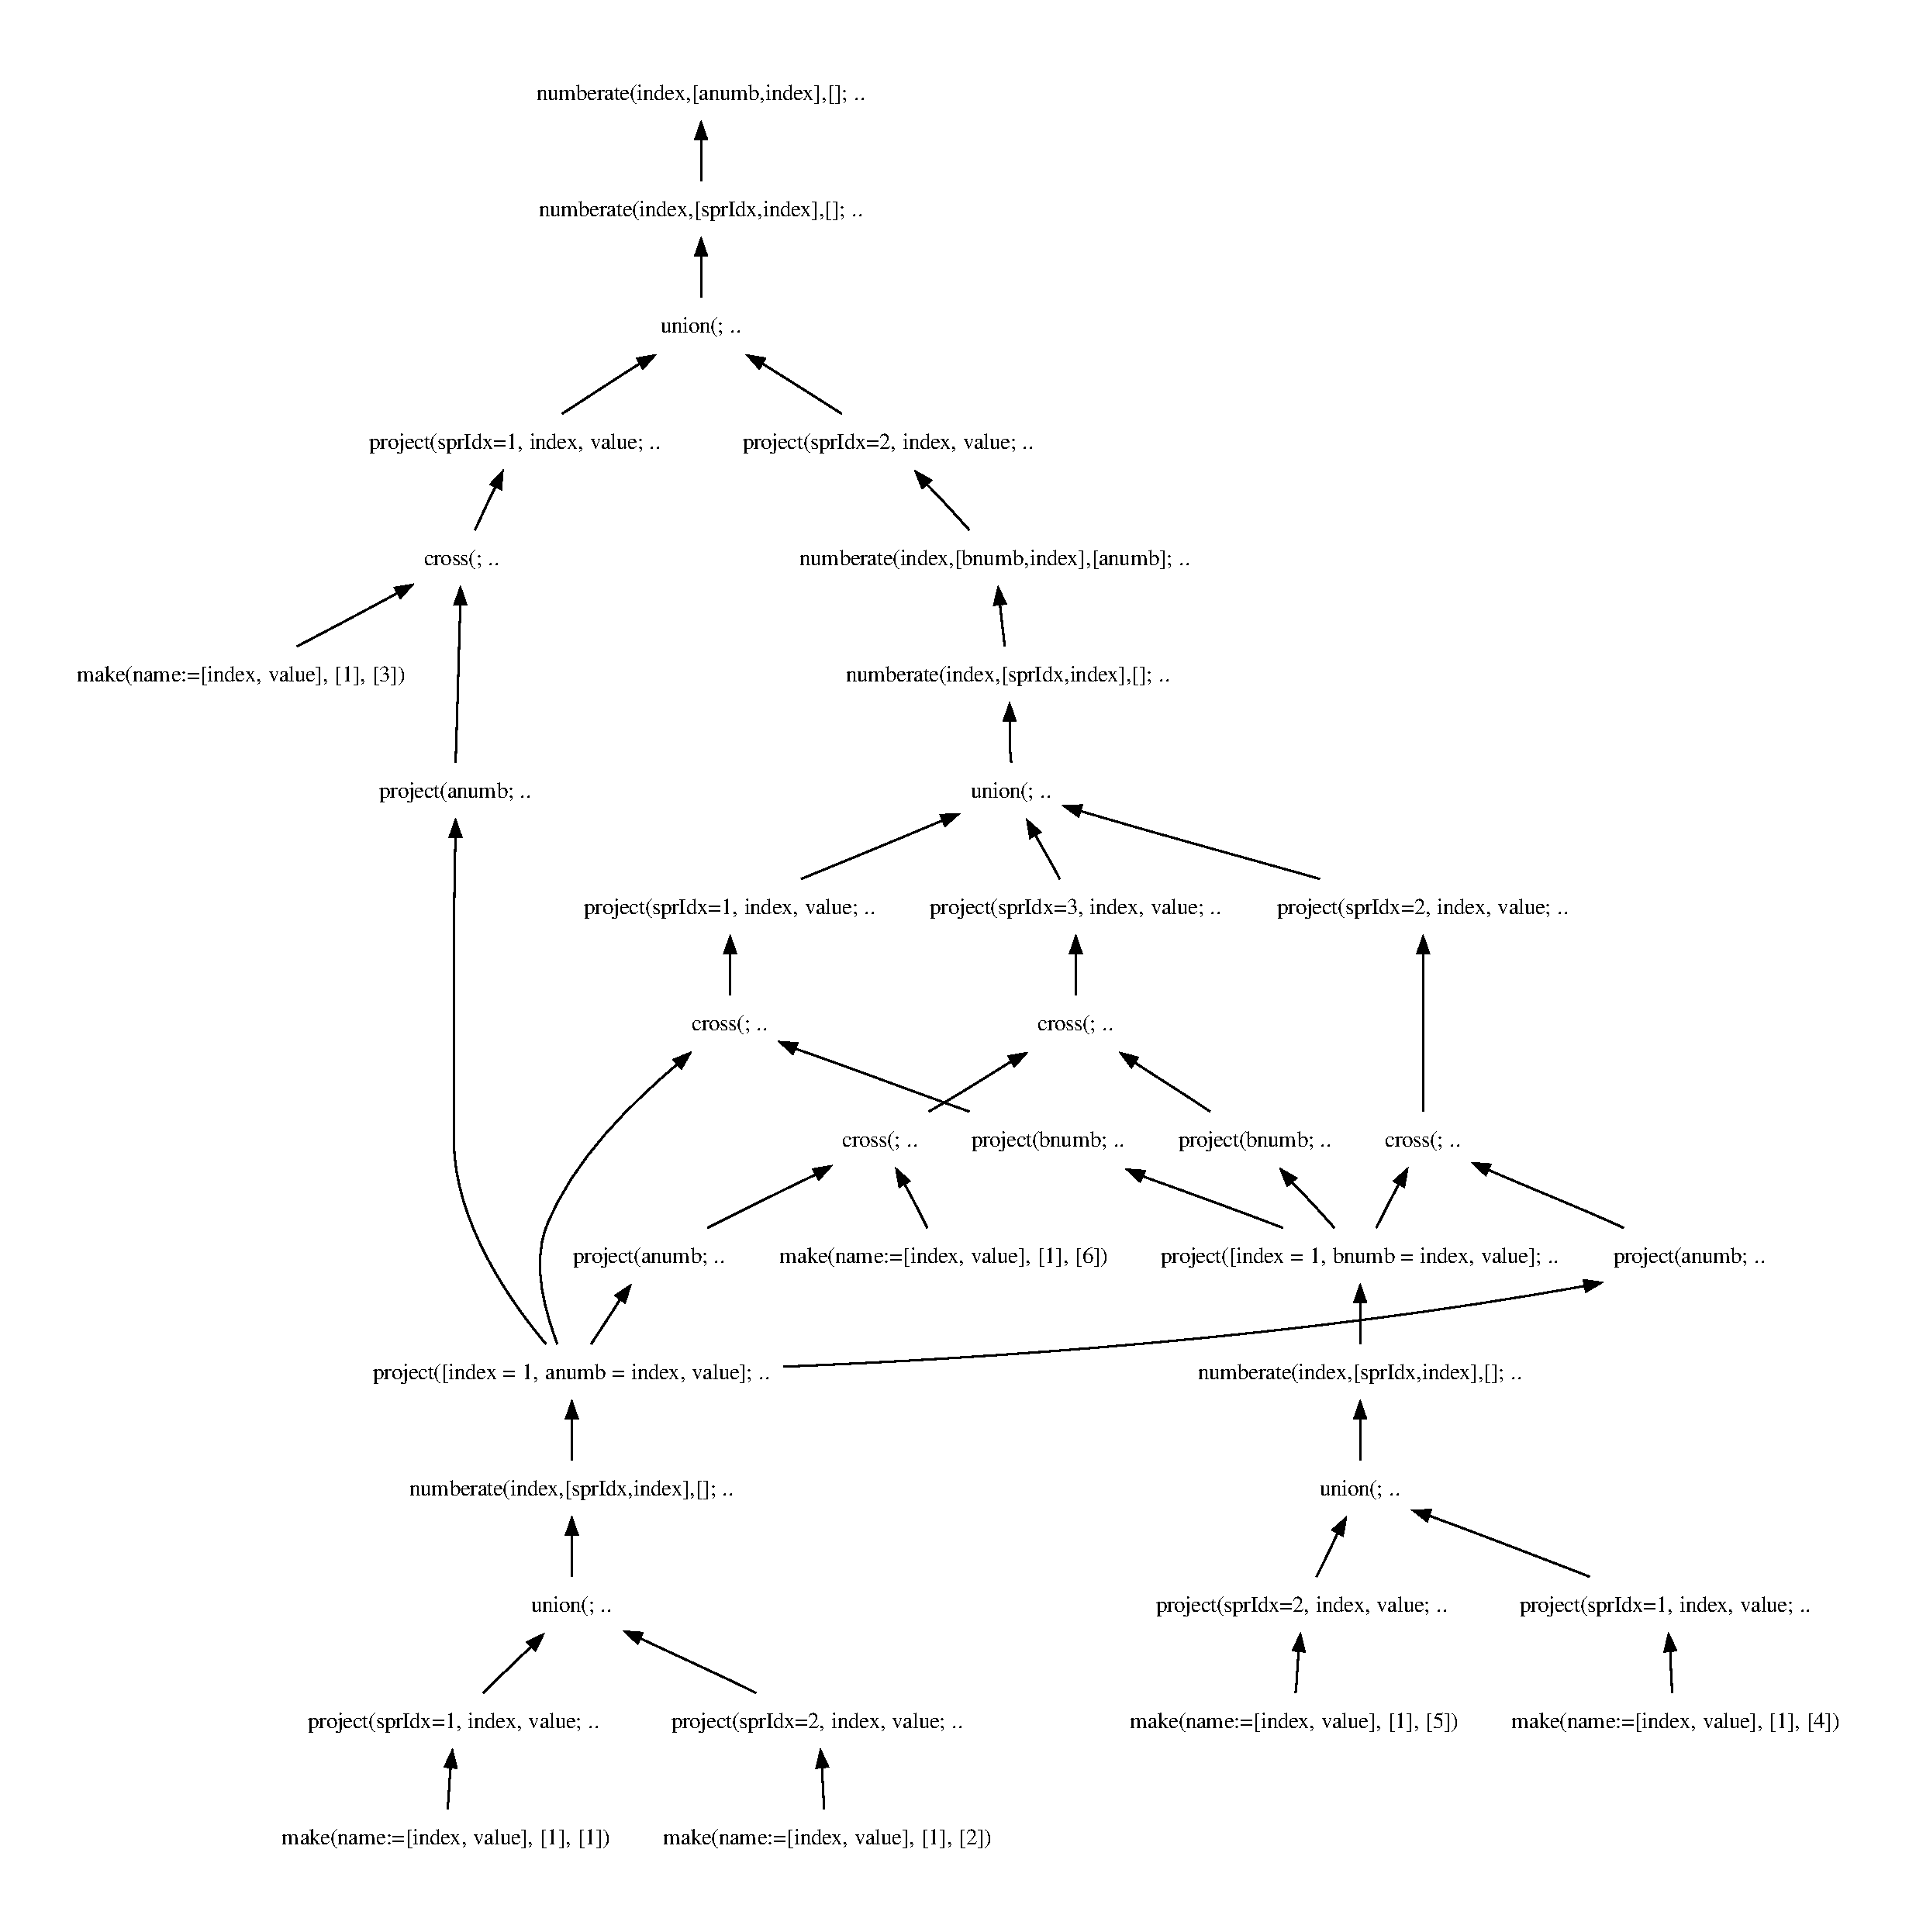
\includegraphics[width=1.0\textwidth]{img/graphs/td_impl_flwor_complex_xq_relalg_dag}
  \caption{Complete translation of expression in figure
  \ref{fig:results:query_complex_flwor} converted to a DAG}
  \label{fig:results:query_complex_flwor_result_dag}
\end{center}
\end{figure}
\newpage

\subsection{FLWOR with conditional}
\label{sect:results:algebra:generated:conditional_flwor}
\subsubsection{Query premise}
\begin{figure}[!htp]
\begin{center}
\begin{Verbatim}
for $a in (10,20) return if ($a > 15) then $a else 15
\end{Verbatim}
  \caption{Conditional FLWOR query premise}
  \label{fig:results:query_conditional_flwor}
\end{center}
\end{figure}

\subsubsection{Result}
\begin{figure}[!htp]
\begin{center}
  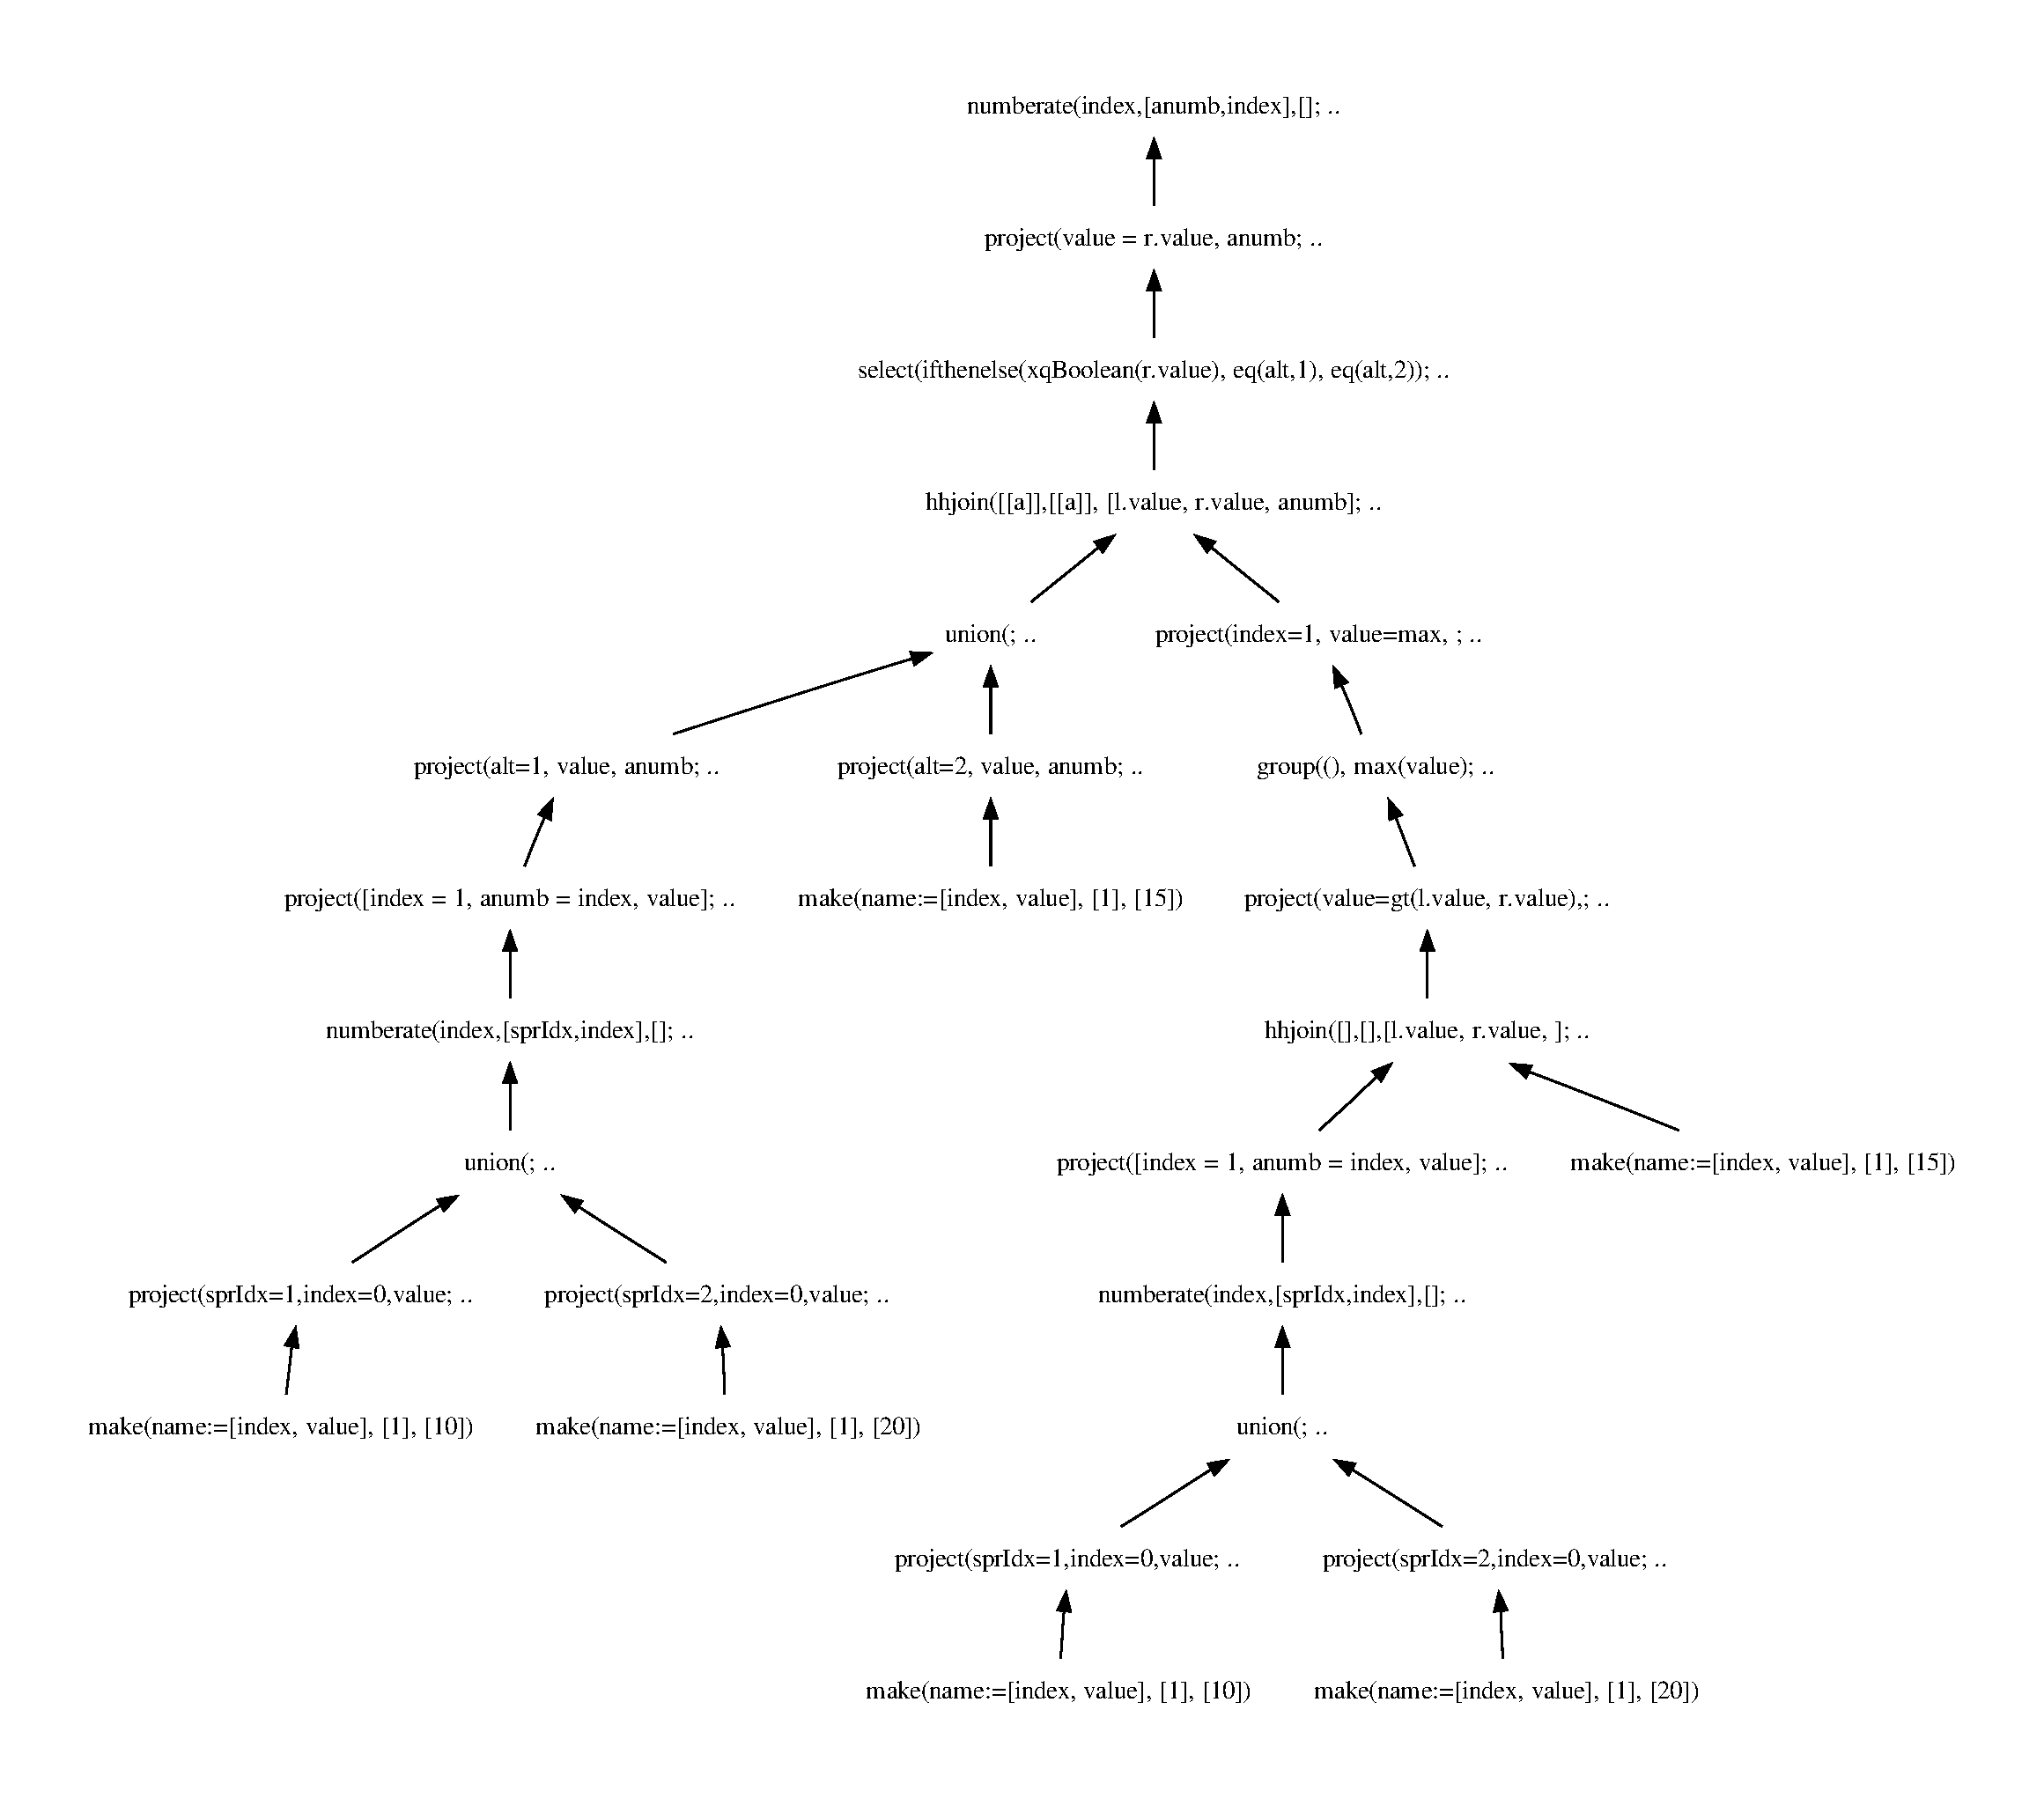
\includegraphics[width=1.0\textwidth]{img/graphs/td_impl_flwor_ifthenelse_xq_relalg}
  \caption{Complete translation of expression in figure
  \ref{fig:results:query_conditional_flwor}}
  \label{fig:results:query_conditional_flwor_result}
\end{center}
\end{figure}

The algebra tree in figure \ref{fig:results:query_conditional_flwor_result} can
be converted to the DAG in figure
\ref{fig:results:query_conditional_flwor_result_dag}

\newpage
\begin{figure}[!htp]
\begin{center} 
  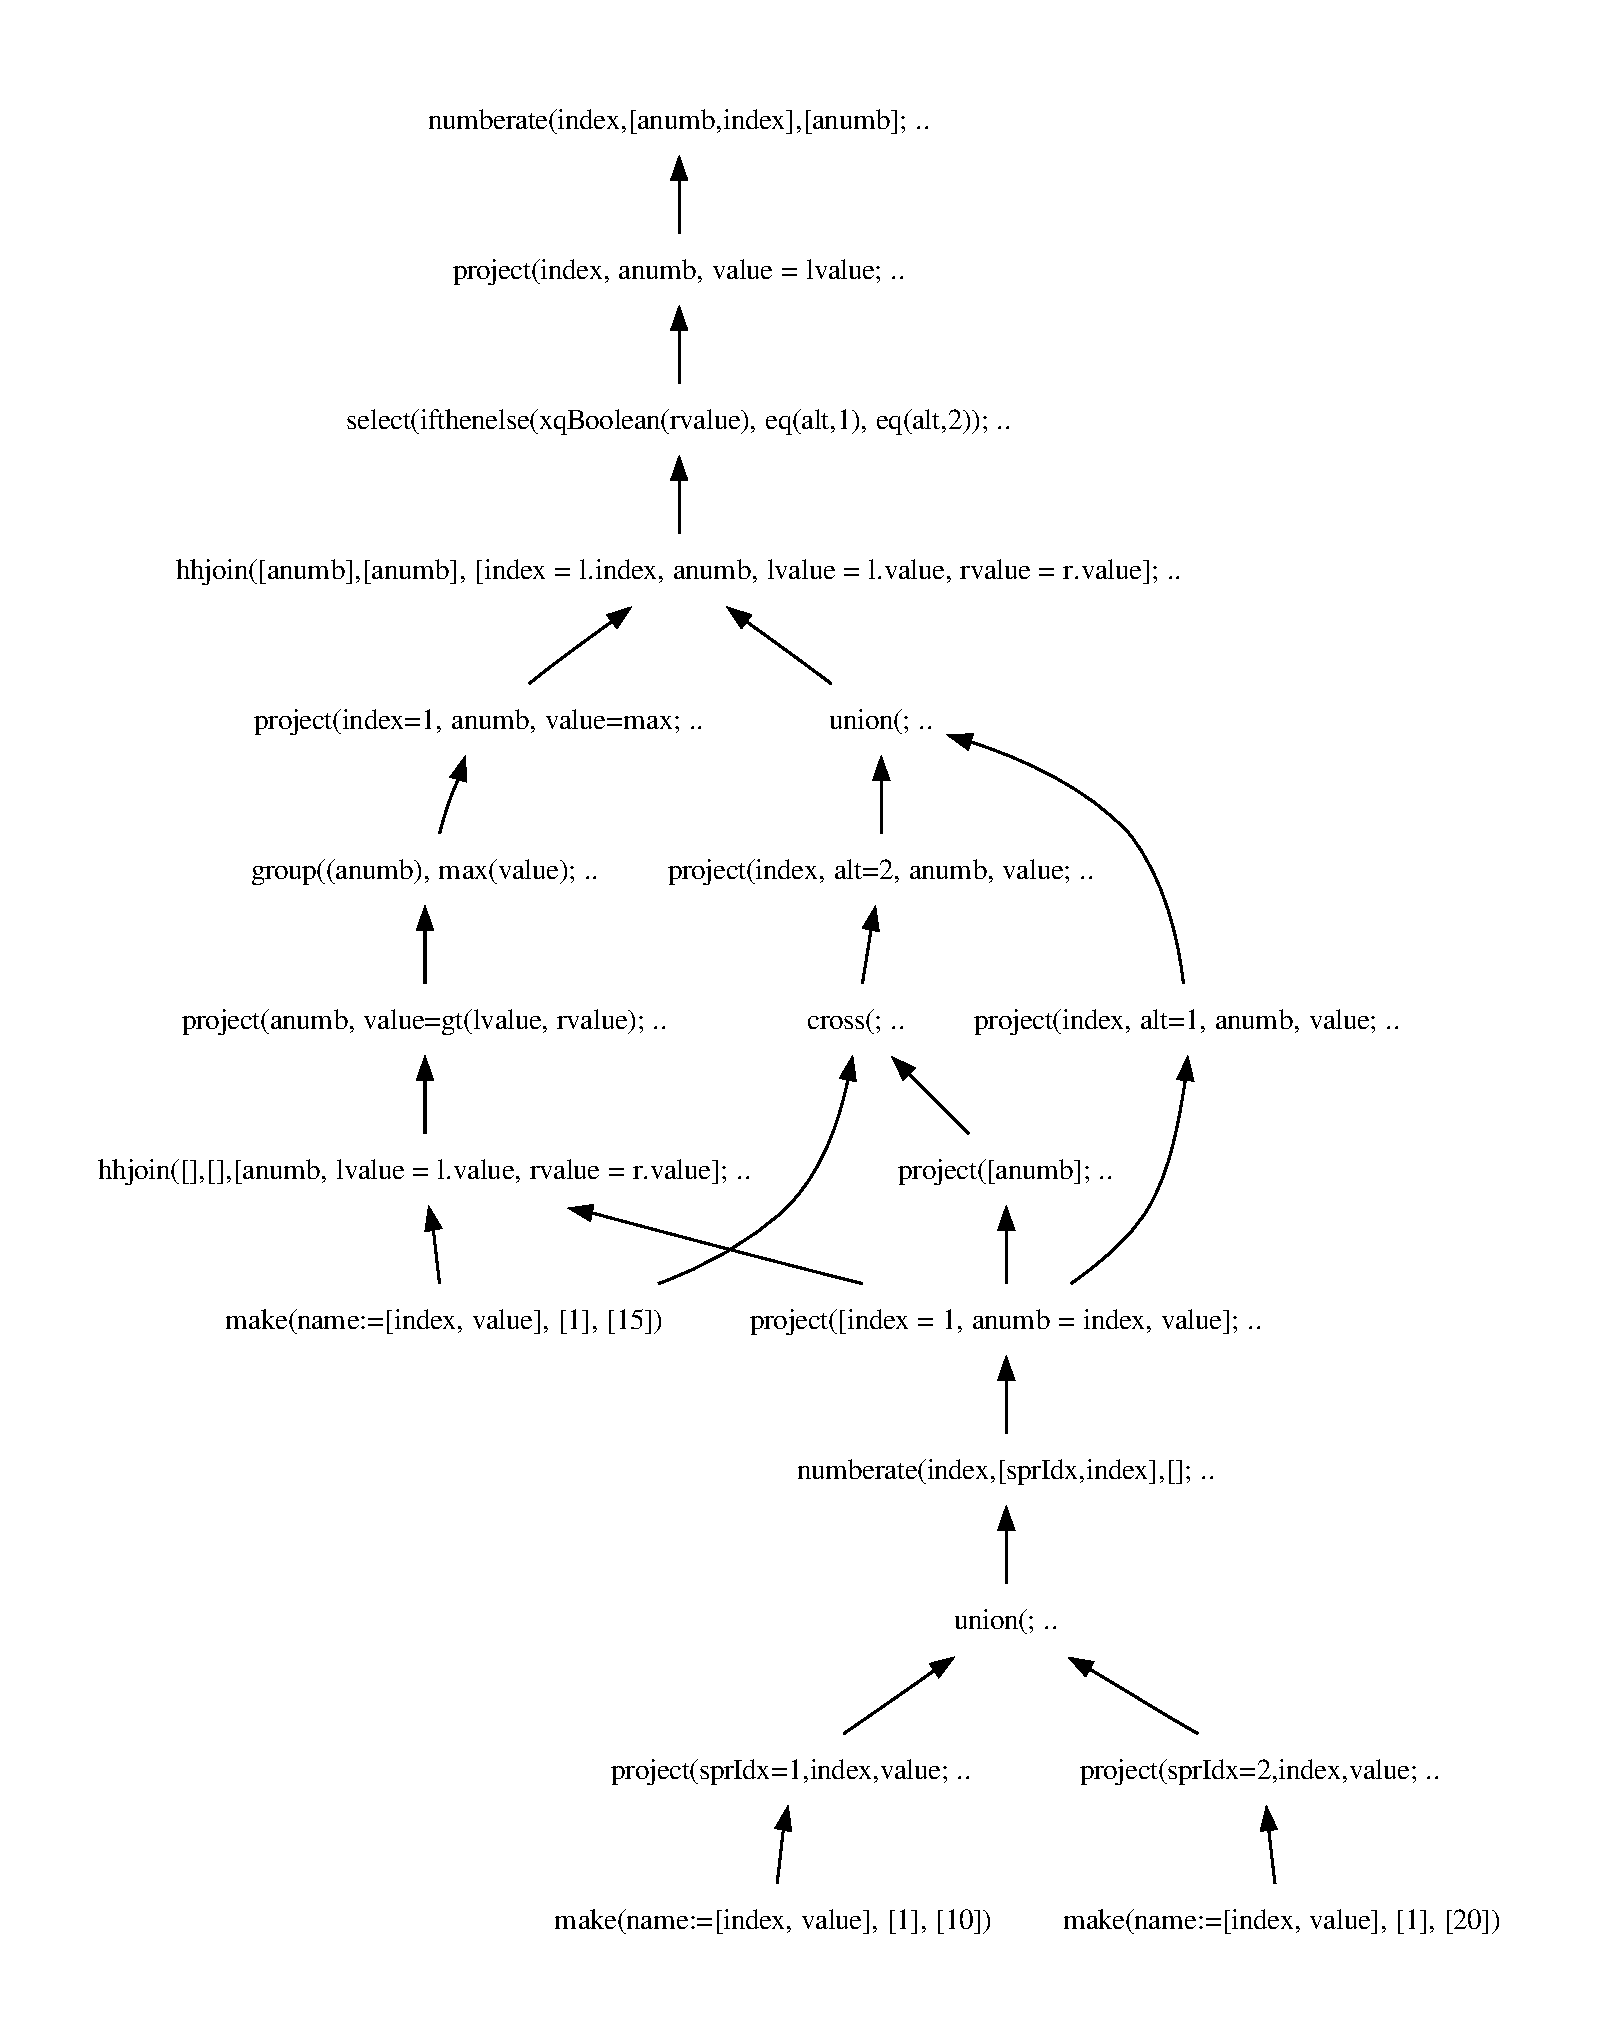
\includegraphics[width=1.0\textwidth]{img/graphs/td_impl_flwor_ifthenelse_xq_relalg_dag}
  \caption{Complete translation of expression in figure
  \ref{fig:results:query_conditional_flwor} converted to a DAG}
  \label{fig:results:query_conditional_flwor_result_dag}
\end{center}
\end{figure}